\section{Android系统架构}
Android系统由多个软件层次构成, 这些层次功能分明, 每一层都对其上的一层提供服务, 构成一个5层的软件栈\juhao 软件栈最底层为Linux内核层, 其上为硬件抽象层, 之后为本地函数库层, 该层次包括了Android Runtime和其他的一些本地函数库, 再上层为Android框架层, 该层包括了提供给应用程序的API和系统管理服务程序, 最上层为应用层, 该层次为用户直接交互的应用程序运行的层次\juhao  图\ref{androidStructure}给出了各层次的组件和关系\juhao
\begin{figure}[ht]
\centering
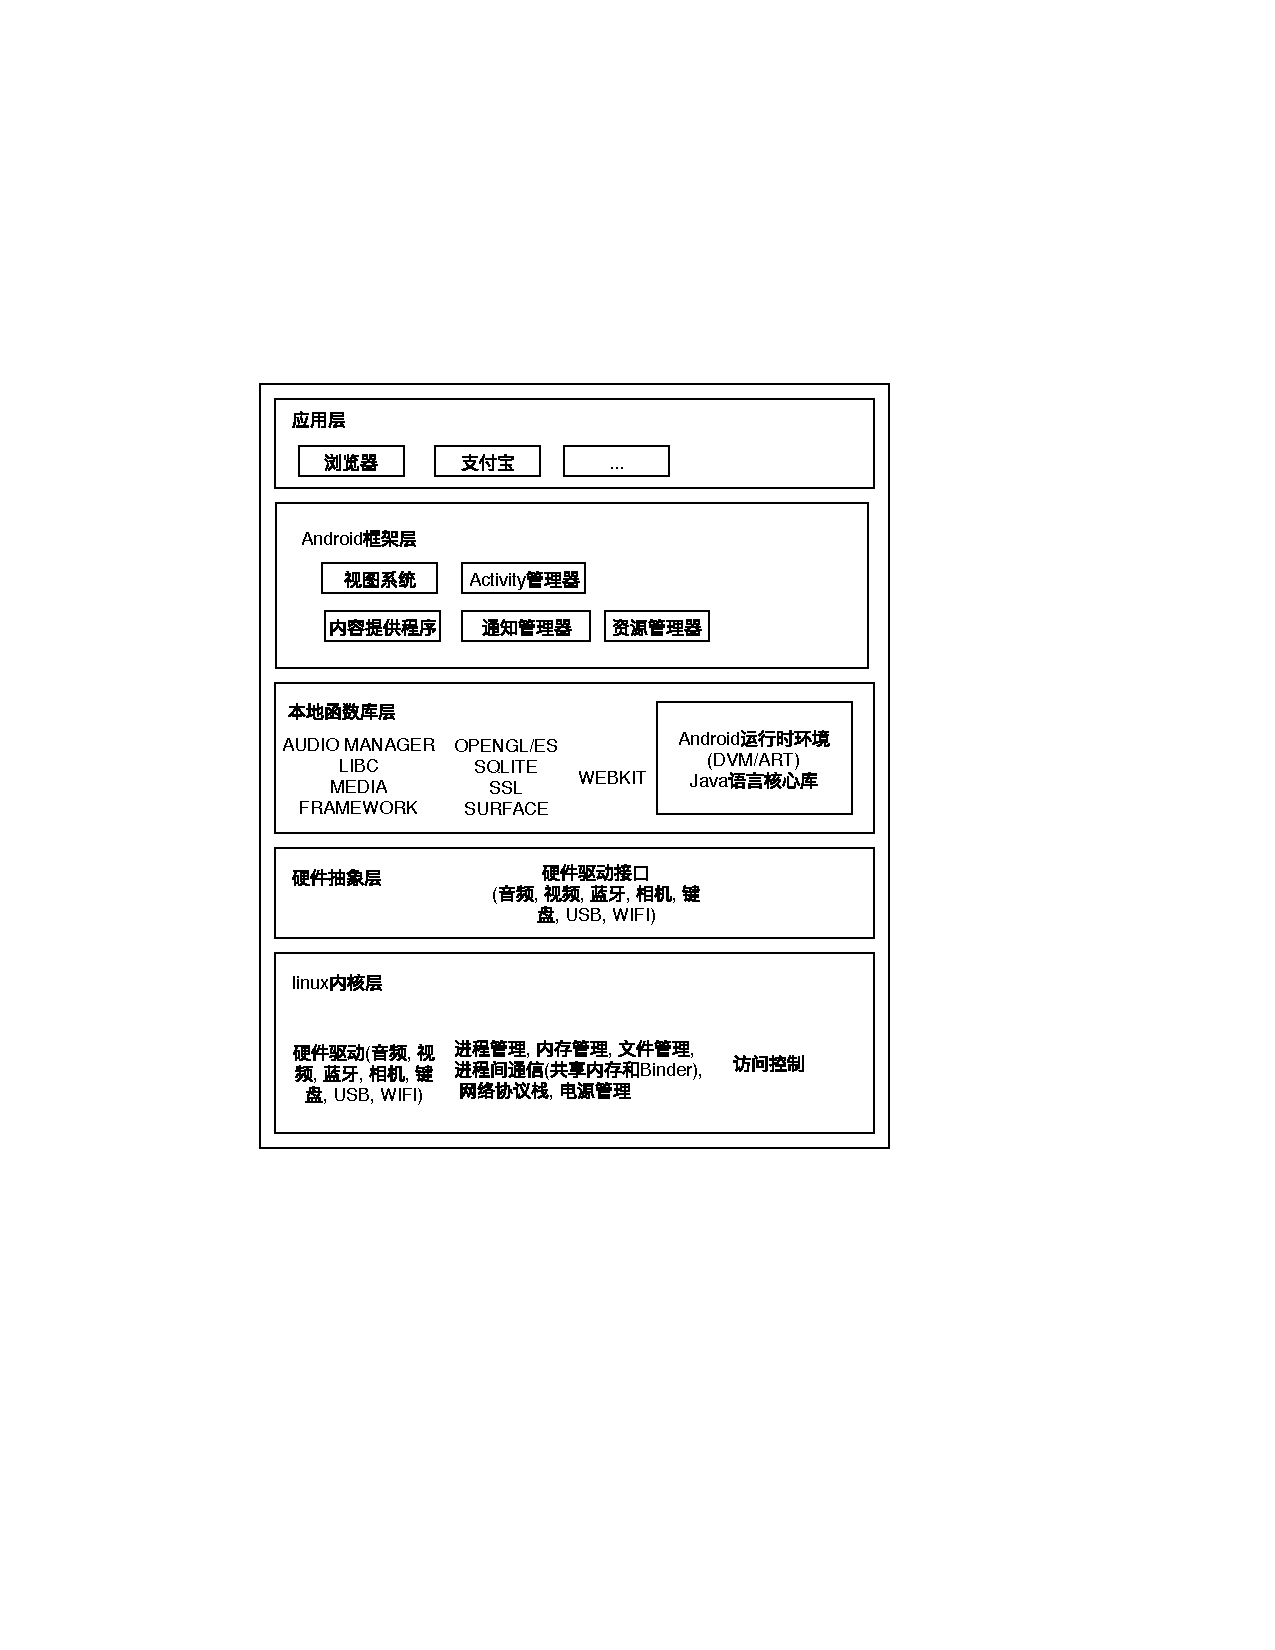
\includegraphics[width=\textwidth]{android_structure.jpg}
\caption{Android系统架构}
\label{androidStructure}
\end{figure}

\subsection*{Linux内核层} 
Android基于修改的Linux内核构建, Linux内核为Android系统提供了操作系统的基本功能, 包括进程管理, 内存管理, 文件管理, 进程间通信(共享内存和Binder), 网络协议栈, 电源管理, 许多设备驱动程序(音频, 视频, 蓝牙, 相机, 键盘, USB, WIFI等)以及访问控制机制(基于用户和用户组的访问控制和selinux)\juhao 这些功能通过系统调用的方式提供给上层使用, 因此, 监控系统调用的使用情况能够获取到应用对关键资源的访问行为\juhao

\subsection*{硬件抽象层}
硬件抽象层是定义了用于更高层次调用对应硬件驱动的接口, 屏蔽了不同厂商的同种设备驱动的差异, 降低Android系统与硬件的耦合度, 便于Android系统的移植\juhao 硬件抽象层包含多个库模块,其中每个模块都为特定类型的硬件组件实现一个接口,例如相机或蓝牙模块。当更高层次要求访问设备硬件时,Android系统将为该硬件组件加载库模块。

\subsection*{本地库层}
本地库层由许多由C/C++开发的系统运行库组成\juhao 这些运行库主要分为两部分, 第一分部为Android运行时环境相关的库, 第二部分为其他系统运行库\juhao 

Android运行时环境由给应用提供Java运行环境的虚拟机实现和实现Java API的核心运行时库组成\juhao 虚拟机实现在Android4.4之前为Dalvik虚拟机, Android4.4时ndroid Runtime(ART)虚拟机作为实验特性加入, 并喝Dalvik虚拟机共存, Android5.0之后只保留了ART虚拟机\juhao Android框架层的许多服务程序和应用层的应用软件就运行在自身的虚拟机实例中\juhao 核心运行时库,可提供Java API框架使用的Java编程语言大部分功能\juhao

其他系统运行库包括许多重要的功能的实现, 主要包括以下部分: 
AUDIO MANAGER用于管理音频输入输出; 
LIBC提供了c语言标准函数库; 
MEDIA FRAMEWORK提供了对常见音频和视频处理的支持; 
OPENGL/ES提供了2D/3D图形绘制功能;
SQLITE提供了访问SQLite数据库的函数;
SSL提供了常见的加密功能;
SURFACE MANAGER提供对显示子系统的支持和管理;
WEBKIT提供了浏览器引擎的实现\juhao

本地库层的各种功能函数除了提供给Android系统自身以实现系统服务功能, 还可以通过Android Native Development Kit(NDK)让应用程序通过Java Native Interface(JNI)调用, 因此对本层函数调用情况的监控可以获取到应用的行为\juhao

\subsection*{Android框架层}
Android框架层包括了许多系统服务程序和组件以及提供给应用程序的访问系统资源的Java API\juhao 这些服务程序和组件主要包括以下几部分:

1. 资源管理器,用于访问非代码资源,例如本地化的字符串、图形和布局文件

2. 通知管理器,可让所有应用在状态栏中显示自定义提醒

3. Activity管理器,用于管理应用的生命周期,提供常见的导航返回栈

4. 内容提供程序,可让应用访问其他应用(例如“联系人”应用)中的数据或者共享其自己的数据

5. 丰富、可扩展的视图系统,可用以构建应用的 UI,包括列表、网格、文本框、按钮甚至可嵌入的网络浏览器

Android框架层是与应用程序联系最紧密的层次, 也是应用程序最容易访问系统资源的层次, 因此对该层次提供的API的监控能够显示应用的主要行为\juhao

\subsection*{应用层}
应用层包括了所有用户直接使用的应用软件,例如电话、短信、浏览器、微信、支付宝等\juhao 这些应用软件主要由Java语言开发, 通过调用Android框架层提供的API和Java语言的标准API实现功能, 每个应用运行于自己独立进程中的虚拟机实例中, 多个应用间借助框架层提供的API通信(进程间通信最终由内核实现)\juhao 利用NDK, 应用也可以实现自己的本地库, 访问Android系统本地库层的开放甚至隐藏的函数, 并通过JNI在应用的Java部分调用自身的本地库中的本地函数\juhao 由于应用能够直接执行本地代码, 增加了应用程序行为涉及的层次, 需要同时在Java层次和本地层次监控应用的执行才能获取到应用的所有行为\juhao

\section{Android应用结构}
Android应用程序主要以Android Package(APK)的文件形式分发和安装\juhao APK文件本质上是一种zip压缩文件, 由多个文件和文件夹组成 其中包含了应用的代码文件、资源文件、证书文件和清单文件, 以apk作为文件后缀名\juhao 图\ref{packageStructure}给出了APK文件的内部结构\juhao
\begin{figure}[ht]
	\centering
	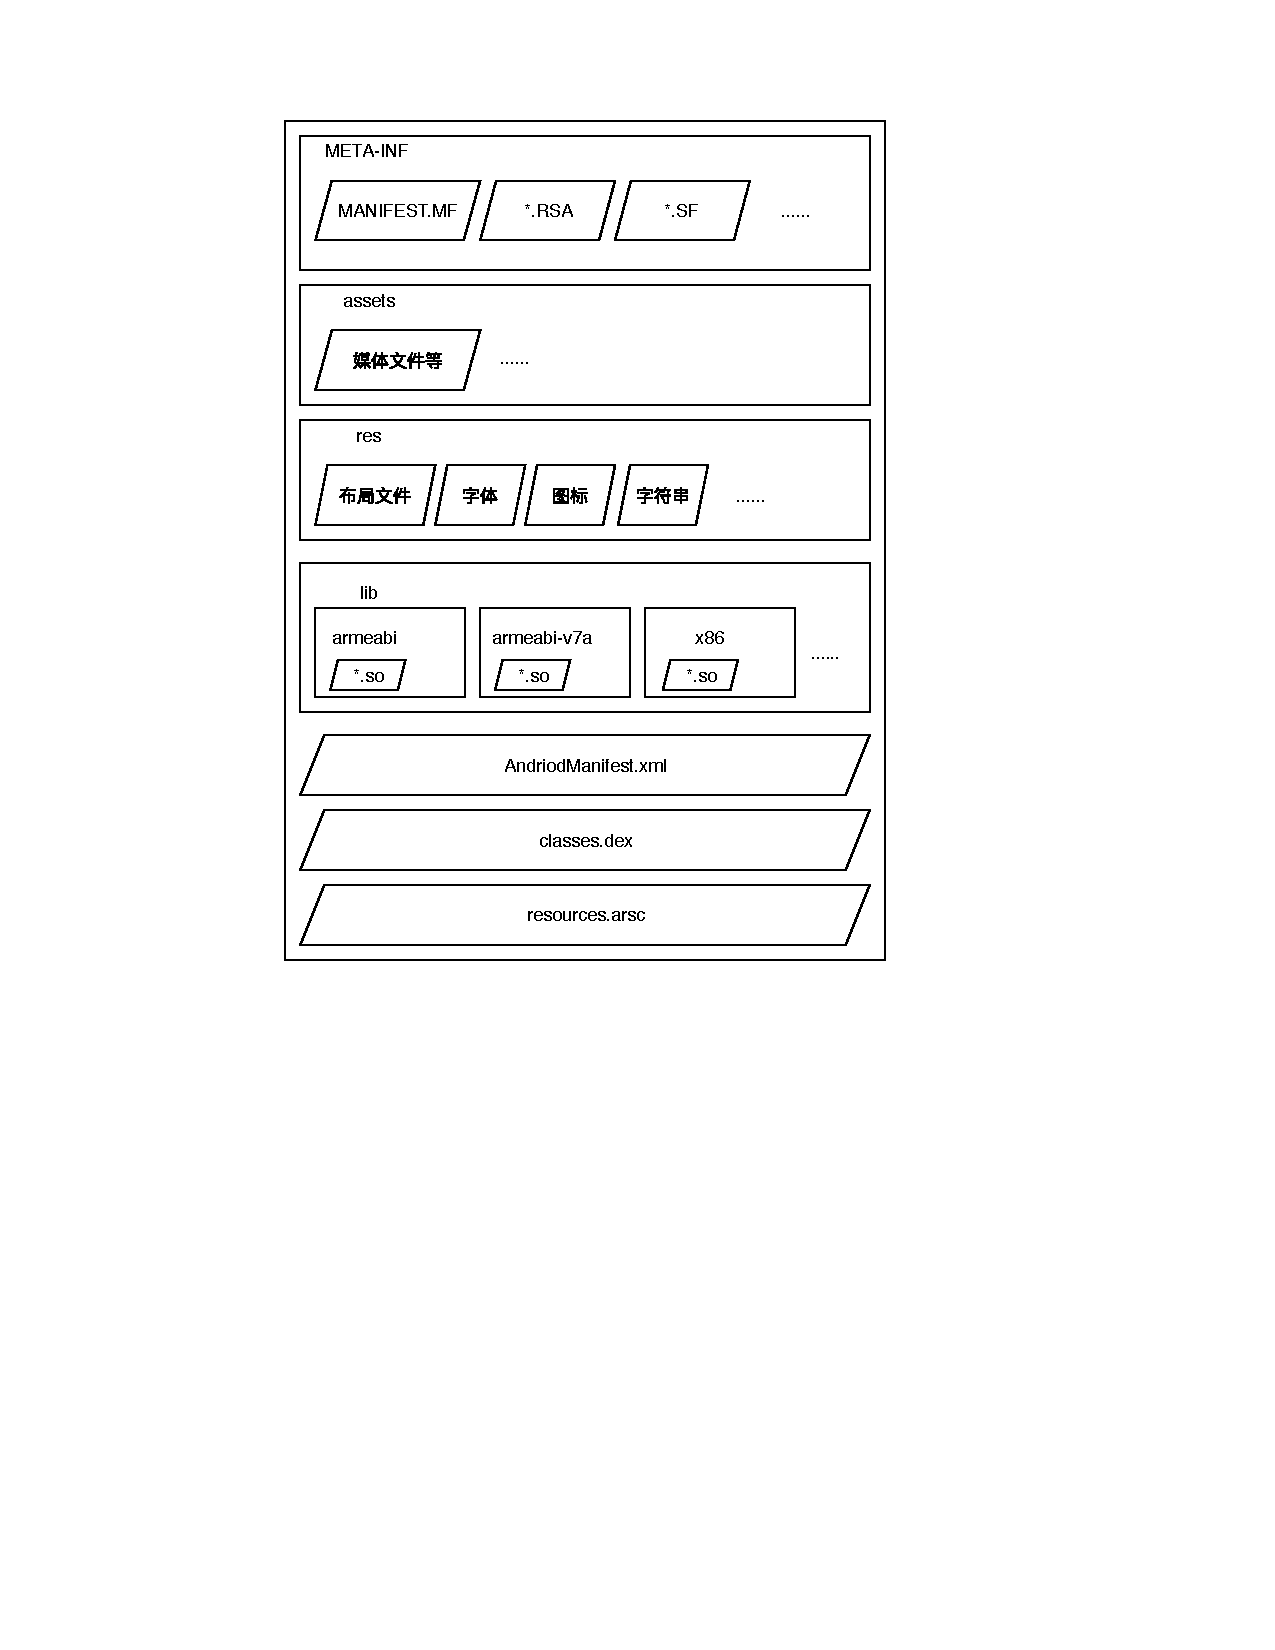
\includegraphics[width=8cm]{package_structure.jpg}
	\caption{APK文件结构}
	\label{packageStructure}
\end{figure}
\paragraph*{META-INF} 
该文件夹包含了与APK文件的签名和校验相关的文件, 一般应该包括至少3个文件:MANIFEST.MF、*.RSA、*.SF(“*”表示文件名不确定)\juhao 
其中MANIFEST.MF记录了APK中的所有文件名和经过base64编码的SHA256校验值(不包括自身);
*.SF记录了MANIFEST.MF文件的经过base64编码的SHA256校验值以及MANIFEST.MF中每一项记录的经过base64编码的SHA256校验值;
*.RSA文件中保存了公钥、所采用的加密算法以及对CERT.SF中的内容的用私钥进行加密之后的值\juhao

\paragraph*{assets} 
该文件夹包括了res中定义类型之外的其他类型的资源文件,例如音频文件,视频文件等媒体文件\juhao 应用还可以把本地库文件放在这个文件里在运行时根据需要动态的加载\juhao

\paragraph*{res}
该文件夹包括了没有编译到resource.arsc中的常用的预定义类型的资源文件\juhao 

\paragraph*{lib}
该文件夹包括了应用的本地库文件, 根据适用的Application Binary Interface(ABI)不同,这些本地库文件会被放在不同的子文件夹里\juhao 当APK被安装时, 系统会选择合适的本地库文件进行安装, 在启动应用时系统会自动加载对应的本地库文件\juhao

\paragraph*{AndroidManifest.xml}
该文件包含了应用的配置信息, 具体来说包含以下几个方面:

1.描述了应用包名;

2.描述了应用的所有组件, 包括构成应用的 Activity、服务、广播接收器和内容提供程序, 以及这些组件可以处理的Intent消息;

3.描述了应用需要使用的权限

4.声明了应用所需的最低Android API级别(与Android版本相对应)

5.列出应用必须链接到的本地库

通过AndroidManifest.xml我们可以得到应用的基本信息\juhao


\paragraph*{classes.dex}
该文件为应用的Java代码编译后的运行于ART或者Dalvik虚拟机的可执行文件\juhao 该文件包含了应用自定义的类的实现代码, 通过反编译该文件可以得到应用的Java源代码, 因此通常会使用加壳和混淆的手段隐藏该文件真正的内容\juhao 对于大型应用, 可能会有多个dex文件\juhao

\paragraph*{resources.arsc}
该文件为编译后的资源文件, 包括xml布局文件, 字符串资源文件等等\juhao


\section{Android动态分析技术}


\section{Android加壳和混淆技术}
\section{Android运行时环境}
\subsection{简介}
\subsection{应用的启动}
\subsection{应用的加载}
\subsection{方法的执行}
\section{Frida}
Frida是一个著名的开源hook框架\juhao

